Qui, di seguito, vengono riportate le architetture relative alla sesta solution. In particolare, come già precedentemente citato, tale solution prevede l'utilizzo della direttiva di partitioning. 
\\
Il partizionamento serve per risolvere un problema tipicamente causato dagli array. Gli array sono implementati come BRAM, solitamente progettate per un dual-port massimo. Questo può limitare il throughput di un algoritmo ad alta intensità di read/write. La larghezza di banda può essere migliorata dividendo l'array (una singola BRAM) in array più piccoli (più BRAM), aumentando di fatto il numero di porte. Gli array vengono partizionati utilizzando la direttiva ARRAY\_PARTITION. Vivado HLS offre tre tipi di partizionamento degli array. I tre tipi di partizionamento sono:
\begin{itemize}
	\item \textbf{block}\\L'array originale viene suddiviso in blocchi di uguali dimensioni di elementi consecutivi dell'array originale.
	\item \textbf{cyclic}\\L'array originale viene suddiviso in blocchi di uguali dimensioni che interlacciano gli elementi dell'array originale.
	\item \textbf{complete}\\L'operazione predefinita consiste nel dividere l'array nei suoi singoli elementi. Ciò corrisponde alla risoluzione di una memoria in registri.
\end{itemize}

\begin{figure}[H]
	\centering
	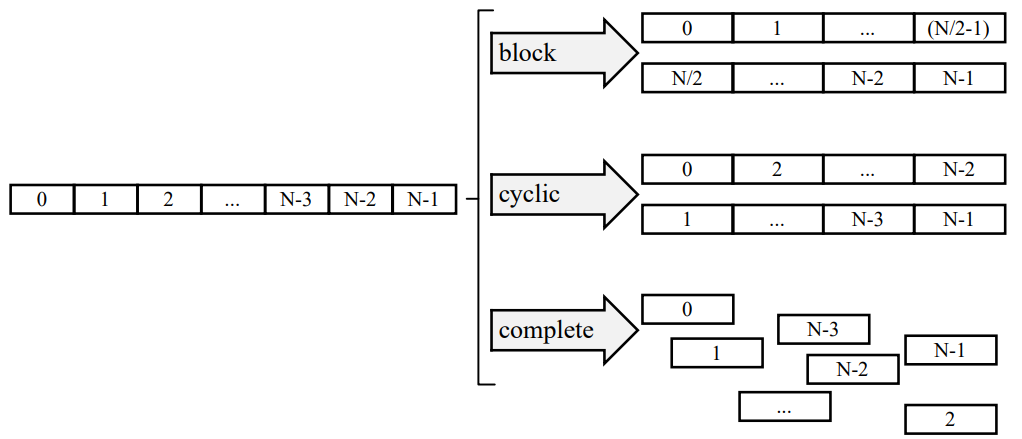
\includegraphics[width=0.5\textwidth]{solutions/s6/partitioning.png}
	\caption{HLS Array Partitioning}
\end{figure}

Nella soluzione hardware in questione verrà utilizzata il partizionamento di tipologia cyclic e nello specifico, verranno analizzate le seguenti implementazioni relative al loop2:
\begin{itemize}
	\item Pipeline, Unroll=2, Cyclic=2 (columnIndex, values, x)
	\item Pipeline, Unroll=2, Cyclic=2 (columnIndex)
	\item Pipeline, Unroll=2, Cyclic=2 (values)
	\item Pipeline, Unroll=2, Cyclic=2 (x)
\end{itemize}

In particolare, è possibile evidenziare nel dettaglio le differenti soluzioni hardware nei seguenti allegati.
\lstinputlisting[language=C++]{solutions/s6/s6all3.cpp}
\lstinputlisting[language=C++]{solutions/s6/s6columnIndex.cpp}
\lstinputlisting[language=C++]{solutions/s6/s6values.cpp}
\lstinputlisting[language=C++]{solutions/s6/s6x.cpp}

Effettuando la sintesi è possibile evidenziare il seguente report:\\

\begin{table}[H]
	\centering
	\begin{tabular}{|c|c|c|c|c|}
		\hline
		\textbf{Solution} & \textbf{Clock} & \textbf{Target} & \textbf{Estimated} & \textbf{Uncertainty} \\
		\hline
		columnIndex, values, x & ap\_clk & 10.00 & 8.510 & 1.25 \\
		\hline
		columnIndex & ap\_clk & 10.00 & 8.510 & 1.25 \\
		\hline
		values & ap\_clk & 10.00 & 8.510 & 1.25 \\
		\hline
		x & ap\_clk & 10.00 & 8.510 & 1.25 \\
		\hline
	\end{tabular}
	\caption{HLS Solution 6 Timing Summary (ns)}
	\label{tab:hls-solution-6-timing-summary}
\end{table}

\begin{table}[H]
	\centering
	\begin{tabular}{|c|c|c|c|c|}
		\hline
		\multicolumn{1}{|c|}{\textbf{Solution}} & \multicolumn{2}{|c|}{\textbf{Latency}} & \multicolumn{2}{|c|}{\textbf{Interval}} \\
		& min & max & min & max \\
		\hline
		columnIndex, values, x & 33 & 41 & 33 & 41 \\
		\hline
		columnIndex & 33 & 41 & 33 & 41 \\
		\hline
		values & 33 & 41 & 33 & 41 \\
		\hline
		x & 33 & 41 & 33 & 41 \\
		\hline
	\end{tabular}
	\caption{HLS Solution 6 Latency Summary (clock cycles)}
	\label{tab:hls-solution-6-latency-summary}
\end{table}

Si può notare come, in corrispondenza di tutte e quattro le soluzioni hardware proposte in questa sezione, i valori di Iteration Latency, trip count, Initiation Interval relativa al loop2 e latenza totale del loop1 e loop2 risultano essere i medesimi. In particolare, il valore di trip count del loop2 risulta essere dimezzato, come quello della solution5, rispetto, ad esempio, alla solution2 dal momento che è presente la direttiva di unrolling di fattore pari a 2. 

\begin{table}[H]
	\centering
	\begin{tabular}{|c|c|c|c|c|c|c|c|c|c|}
		\hline
		\multicolumn{1}{|c|}{\textbf{Solution}} & \multicolumn{1}{|c|}{Loop Name} & \multicolumn{2}{|c|}{\textbf{Latency}} & \multicolumn{1}{c|}{\textbf{Iteration Latency}} & \multicolumn{2}{c|}{\textbf{Initiation Interval}} & \multicolumn{1}{c|}{\textbf{Trip}}  \\
		&  & min & max & & achieved & target & \textbf{Count} \\
		\hline
		columnIndex, values, x & - loop1 & 32 & 40 & 8$\sim$10 & - & - & 4 \\
		& + loop2 & 4 & 6 & 5 & 1 & 1 & 0$\sim$2 \\
		\hline
		columnIndex & - loop1 & 32 & 40 & 8$\sim$10 & - & - & 4 \\
		& + loop2 & 4 & 6 & 5 & 1 & 1 & 0$\sim$2 \\
		\hline
		values & - loop1 & 32 & 40 & 8$\sim$10 & - & - & 4 \\
		& + loop2 & 4 & 6 & 5 & 1 & 1 & 0$\sim$2 \\
		\hline
		x & - loop1 & 32 & 40 & 8$\sim$10 & - & - & 4 \\
		& + loop2 & 4 & 6 & 5 & 1 & 1 & 0$\sim$2 \\
		\hline
	\end{tabular}
	\caption{HLS Solution 6 Latency Loops Summary }
	\label{tab:hls-solution-6-loop-summary}
\end{table}

\begin{table}[H]
	\centering
	\begin{tabular}{|c|c|c|c|c|}
		\hline
		\textbf{Solution} & \textbf{BRAM\_18K} & \textbf{DSP48E} & \textbf{FF} & \textbf{LUT} \\
		\hline
		columnIndex, values, x & 0 & 6 & 535 & 623 \\
		\hline
		columnIndex & 0 & 6 & 533 & 472 \\
		\hline
		values & 0 & 6 & 533 & 472 \\
		\hline
		x & 0 & 6 & 599 & 463 \\
		\hline
	\end{tabular}
	\caption{HLS Solution 6 Utilization Estimates [\#]}
	\label{tab:hls-solution-6-utilization-report}
\end{table}

Si può evidenziare come i valori di latenza associati alle quattro solution proposte risultano essere i medesimi di quelli otteenuti in corrispondenza della soluzione hardware 5.

\begin{table}[H]
	\centering
	\begin{tabular}{|c|c|c|c|c|c|c|c|c|}
		\hline
		\multicolumn{1}{|c|}{\textbf{Solution}} & \multicolumn{1}{|c|}{RTL} & \multicolumn{1}{|c|}{Status} & \multicolumn{3}{c|}{\textbf{Latency}} & \multicolumn{3}{c|}{\textbf{Interval}} \\
		& &  & min & avg & max & min & avg & max \\
		\hline
		columnIndex, values, x & VHDL & Pass & 37 & 37 & 37 & NA & NA & NA \\
		\hline
		columnIndex & VHDL & Pass & 37 & 37 & 37 & NA & NA & NA \\
		\hline
		values & VHDL & Pass & 37 & 37 & 37 & NA & NA & NA \\
		\hline
		x & VHDL & Pass & 37 & 37 & 37 & NA & NA & NA \\
		\hline
	\end{tabular}
	\caption{HLS Solution 6 C/RTL Cosimulation Report }
	\label{tab:hls-solution-6-cosimulation-report}
\end{table}

Si può notare come, in corrispondenza della soluzione basata su partitioning dell'array \textit{columnIndex} e dell'array \textit{values} si ha la medesima utilizzazione dei FF. Molto probabilmente questo risultato è legato al fatto che entrambi gli array presentano medesima dimensione, cioè pari a \textit{nnz}. Inoltre, la minore utilizzazione delle risorse si ha in corrispondenza dell'array \textit{x} a cui corrisponde, infatti, la dimensione minore tra i tre array considerati. In particolare, la soluzione in cui viene considerato il partizionamento dei tre array potrebbe essere considerata come la solution che richiede più risorse dal momento che presenta il maggior numero di slice utilizzate.

\begin{table}[H]
	\centering
	\begin{tabular}{|c|c|c|c|c|c|c|c|c|}
		\hline
		\textbf{Solution} & \textbf{SLICE} & \textbf{LUT} & \textbf{FF} & \textbf{DSP} & \textbf{BRAM} & \textbf{CP} & \textbf{CP} & \textbf{CP} \\
		& & & & & & \textbf{required} & \textbf{achieved} & \textbf{achieved}\\
		& & & & & & & \textbf{post-} & \textbf{post-}\\
		& & & & & & & \textbf{synthesis} & \textbf{implementation}\\
		\hline
		columnIndex, values, x  & 113 & 316 & 198 & 6 & 0 & 10 & 7.927 & 7.799 \\
		\hline
		columnIndex  & 84 & 259 & 224 & 6 & 0 & 10 & 7.472 & 7.843 \\
		\hline
		values  & 99 & 327 & 224 & 6 & 0 & 10 & 7.502 & 8.184 \\
		\hline
		x  & 99 & 250 & 198 & 6 & 0 & 10 & 6.541 & 6.931 \\
		\hline
	\end{tabular}
	\caption{HLS Loop Unrolling Factor=2 Solution Export RTL Report}
	\label{tab:hls-solution-6-export-rtl-report}
\end{table}